\documentclass[11pt,a4j,fleqn]{jarticle}
\usepackage{amsmath,amsthm,amssymb}
\usepackage[dvipdfmx]{graphicx}
\usepackage{float}

\title{尾山ゼミ演習課題\\Pythonによる包絡線定理作図のレポート}
\author{荘 直哉}
\date{2014年6月7日}


\begin{document}

\maketitle

\section{はじめに}

以下は、2014年5月に尾山ゼミにて行ったPythonを用いた演習のレポートである。Pythonを利用し、包絡線定理の図を作成した。


\section{包絡線定理}
ある関数$f(x,t)$のパラメータ$t$を動かして得られる直線群又は曲線群に対し、共通して接している曲線のことを包絡線(Envelope)という。
今回は、以下に定義される直線$y=f(x, t) = tx - t^2$のパラメータ$t$を動かし、包絡線を作図した。包絡線定理の詳細については、尾山・安田~\cite{OyamaYasuda11}などを参照されたい。

\section{出力結果}
出力結果は以下。図1では、$t$を-4から4の範囲で15回、図2では-5から5の範囲で30回動かしている。

\begin{figure}[!b]
  \centering
  \begin{minipage}{0.4\columnwidth}
    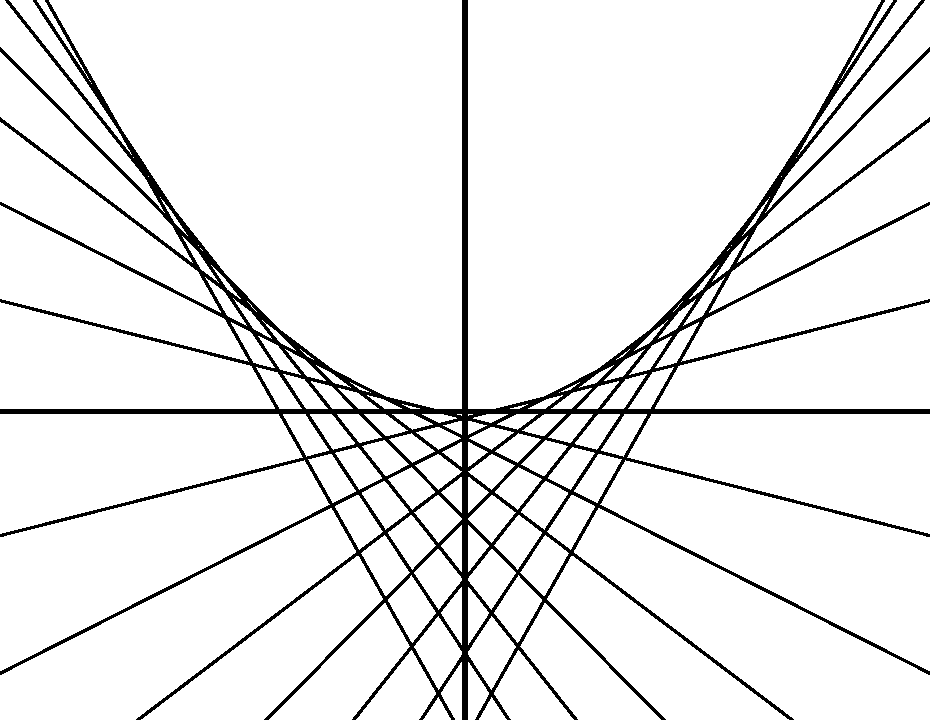
\includegraphics[width=0.3\columnwidth]{envelope0.pdf}
    \caption{直線が少なめの例}
    \label{fig:1}
  \end{minipage}
  \hspace{1cm}
  \begin{minipage}{0.4\columnwidth}
    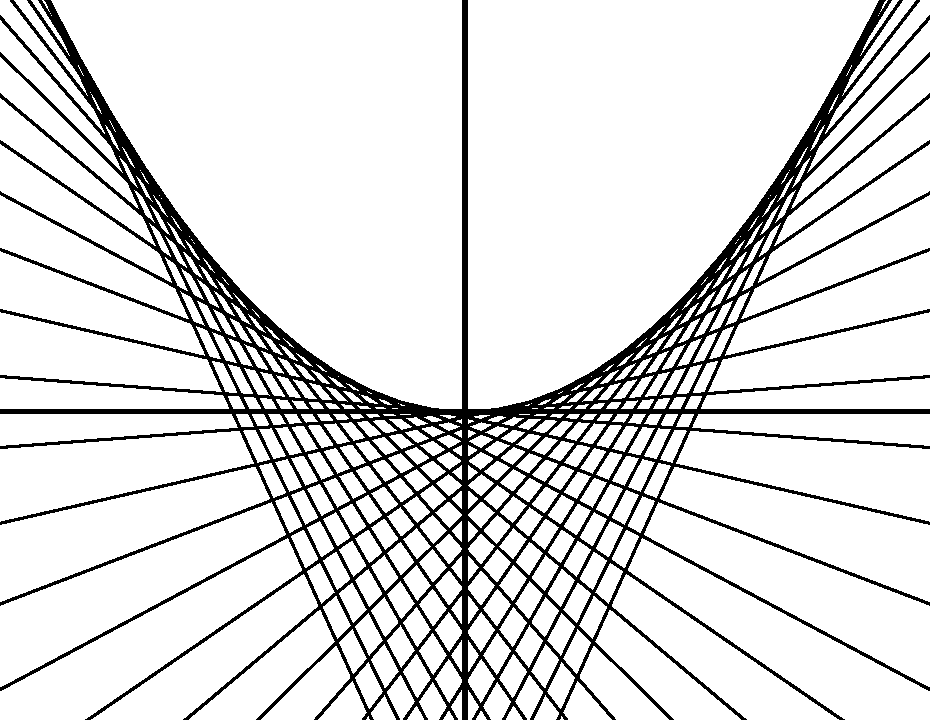
\includegraphics[width=0.3\columnwidth]{envelope1.pdf}
    \caption{直線が多めの例}
    \label{fig:2}
  \end{minipage}
\end{figure}

\newpage

\section{Pythonプログラム}

上記図表を描画するPythonコードは下記の通りである。包絡線の式のパラメータ\texttt{t}を\texttt{for}ループによって動かし、プロットすることで作成。
\texttt{switch}によって、\texttt{t}を動かす範囲と幅(繰り返しの回数)を2パターンのうちから選んでいる。
画像の保存については、\texttt{plt.savefig()}によって行い、\texttt{for FORMAT in ['.png', '.pdf']:} のように\texttt{for}ループを設定することで、pngとpdfの2つの形式で自動的に保存した。


\begin{quote}
\begin{verbatim}
import numpy as np
import matplotlib.pyplot as plt

# 包絡線の式
def f(x, t):
    return t * x - t**2

#グラフの軸などの設定
def subplots():
    fig, ax = plt.subplots()

    for spine in ['left', 'bottom']:
        ax.spines[spine].set_position('zero')
        
    for spine in ['right', 'top']:
        ax.spines[spine].set_color('none') 

    ax.set_xticks([])
    ax.set_yticks([]) 
    
    return (fig, ax)

fig, ax = subplots() 

# xの定義域を設定
x = np.linspace(-50,50,1000)

# x,yの表示範囲を設定
ymin =-15
ymax =20
xmin =-10
xmax =10
v = [xmin, xmax, ymin, ymax]

switch = 0 # 包絡線の本数を設定 (0 or 1)

if switch == 0:
	slopes = np.linspace(-4,4,15)#パラメータを動かす範囲と回数
if switch == 1:
	slopes = np.linspace(-5,5,30)

for slope in slopes:
    y = f(x, t=slope)
    plt.plot(x, y, 'k-')
plt.axis(v)
plt.axvline(linewidth=2, color='k') #x軸の設定
plt.axhline(linewidth=2, color='k') #y軸の設定
for FORMAT in ['.png', '.pdf']:
	plt.savefig('envelope'+ str(switch) +FORMAT,transparent=True, bbox_inches='tight', pad_inches=0)
plt.close()

\end{verbatim}
\end{quote}


\begin{thebibliography}{0}
\bibitem{OyamaYasuda11}
尾山大輔・安田洋祐「経済学で出る包絡線定理」『経済セミナー』2011年10・11月号.
\end{thebibliography}

\end{document}